\documentclass[10pt,a4paper]{article}
\usepackage[margin=2.2cm]{geometry}
\usepackage{fontspec}
\usepackage{kotex}
\setmainfont{Apple SD Gothic Neo}
\setsansfont{Apple SD Gothic Neo}
\usepackage{amsmath,amssymb}
\usepackage{graphicx}
\usepackage{booktabs}
\usepackage{caption}
\usepackage[dvipsnames]{xcolor}
\usepackage[colorlinks=true,linkcolor=MidnightBlue,citecolor=MidnightBlue,
            urlcolor=MidnightBlue]{hyperref}
\usepackage{titlesec}
\titleformat{\section}{\large\bfseries}{\thesection}{0.6em}{}
\titleformat{\subsection}{\normalsize\bfseries}{\thesubsection}{0.5em}{}
\captionsetup{font=small,labelfont=bf}
\setlength{\parskip}{0.35em}
\setlength{\parindent}{0pt}

\usepackage{mdframed}
\newmdenv[linewidth=0.4pt,linecolor=gray!60,backgroundcolor=gray!5,
          innertopmargin=6pt,innerbottommargin=6pt,skipabove=8pt,skipbelow=8pt]{claimbox}
\newcommand{\claim}[2]{\begin{claimbox}\textbf{주장.} #1\par\smallskip
  \textcolor{gray!70}{\textbf{반증 조건.} #2}\end{claimbox}}

\title{\bfseries 어제 만든 자가 오늘 나를 막았다\\[2pt]
\large 임베딩은 붕괴하지 않고 축은 11/11 에 붙었는데, 얇은 셋의 문턱은 판 문턱의 3.5배였다}
\author{월드모델 실험실 · 노트 720 · 721}
\date{2026-08-06}
\begin{document}\maketitle

\section{한 줄}

사용자 제안(\emph{``공유 인코더 + 도메인별 토큰''})의 두 번째 단계를 쟀다.
\textbf{도메인 임베딩이 붕괴하지 않았고}(짝 코사인 최대 $0.648$, 문턱 $0.95$)
\textbf{축이 11개 도메인 전부에 붙었다}. 그런데 판을 못 움직인다 --- 판 신호 몫
$+0.0106$ 이고 \textbf{유보 126행 도메인 하나를 빼면 $+0.0038$ 로 문턱 미달}이다.
그리고 하마터면 ``얇은 셋이 문턱을 넘었다''고 쓸 뻔했다 --- \textbf{몇 시간 전에
만든 법칙이 그것을 막았다.}

\section{물음은 노트 698 이 좁혀 놨다}

노트 698 이 첫 단계(공유 어휘 $+$ 공유 가중)를 닫았다 --- 신호 몫 $+0.0040 <$ 문턱
$0.0045$ 이고 \textbf{시장팝업 하나를 빼면 $-0.0018$ 로 뒤집혔다}. 진단은
\emph{``공유가 덮음을 사고 정확도를 판다''}였다(축이 8$\to$10 도메인에 붙었는데
가중 최대인 웹툰이 $-0.0190$).

그 실패가 물음을 정확하게 만들었다. \textbf{도메인별 차이가 실재함이 확인됐으므로}
(웹툰 $-0.0190$ 대 시장팝업 $+0.1534$) 물음은 ``공유가 되나''가 아니라
\textbf{``임베딩 8차원이 그 차이를 담을 수 있나''}다.

\begin{figure}[t]\centering
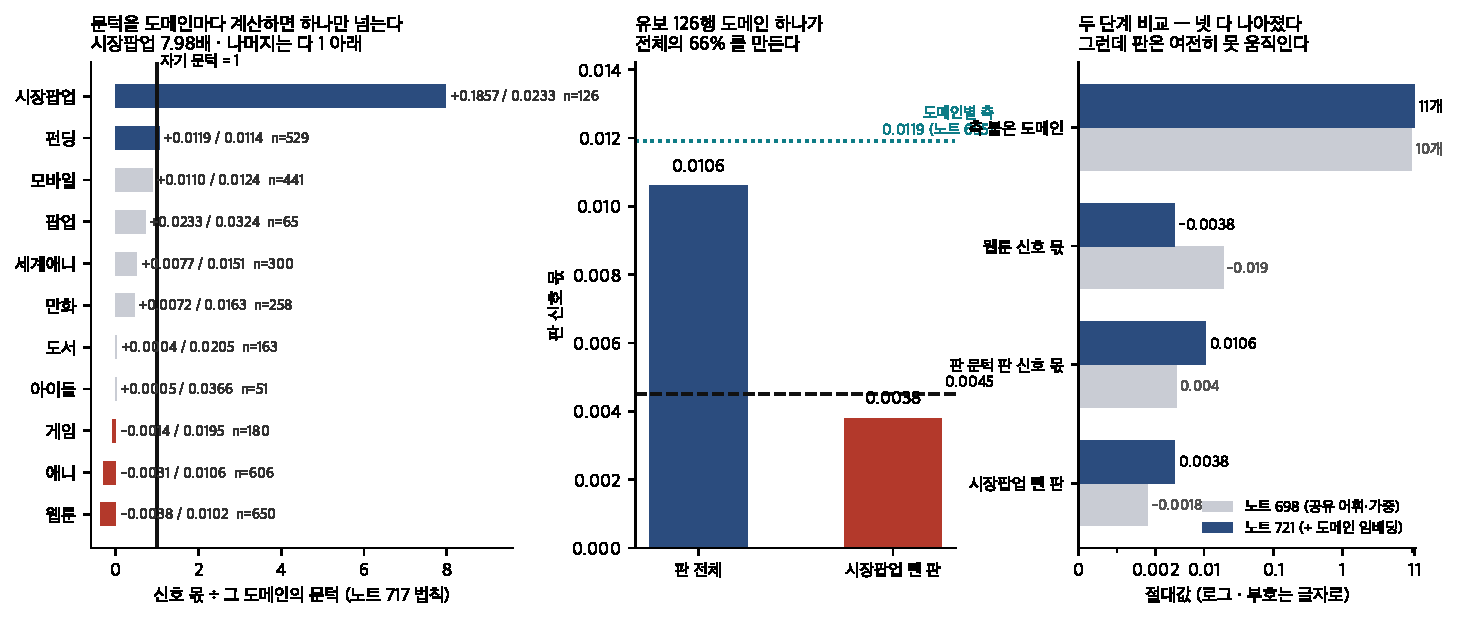
\includegraphics[width=0.99\textwidth]{figs/yesterday.pdf}
\caption{왼쪽: \textbf{문턱을 도메인마다 계산하면 하나만 넘는다.} 가운데: 유보
126행 도메인 하나가 판 신호 몫의 $66\%$ 를 만든다. 오른쪽: 두 단계 비교 ---
\textbf{넷 다 나아졌는데 판은 여전히 안 움직인다.}}
\end{figure}

\section{담을 수 있다 --- 그리고 축이 전 도메인에 붙는다}

\begin{center}
\begin{tabular}{lll}
\toprule
판정 (노트 685 가 미리 못박음) & 결과 & \\
\midrule
(다) 임베딩 붕괴 안 하나 & 코사인 최대 $\mathbf{0.648}$ (문턱 $0.95$) & \textbf{통과} \\
(가) 얇은 셋에 축이 붙나 & 팝업 · 아이돌 · 도서 \textbf{셋 다} & \textbf{통과} \\
(가) 그 셋 신호 몫 양수인가 & $+0.0058$ 이지만 \textbf{자기 문턱의 $0.37$배} & \textbf{미달} \\
(나) $+0.0119$ 를 넘나 & $+0.0106$ & \textbf{미달} \\
\bottomrule
\end{tabular}
\end{center}

\claim{\textbf{임베딩 8차원이 도메인 차이를 담는다.} 11개 도메인의 짝 코사인이
평균 $-0.06$ · 최대 $0.648$ 로 서로 다른 방향을 배웠다. 그리고 \textbf{축이 11/11 에
붙어} 팝업(학습 17행) · 아이돌 · 도서까지 예보를 받는다 --- 노트 698 에서는
아이돌이 안 붙었다. \textbf{행 병목은 배선 수준에서 뚫렸다.}}
{임베딩 차원을 $8 \to 4 \to 2$ 로 줄여도 코사인이 계속 낮으면 ``담았다''가 아니라
``차원이 남아 흩어졌다''일 수 있다. 그 경우 축의 신호 몫은 안 변해야 한다 ---
변하면 흩어짐 자체가 일하고 있었다는 뜻이다.}

\section{그런데 어제 만든 자가 나를 막았다}

얇은 셋의 신호 몫이 $+0.0058$ 이고 \textbf{판 문턱 $0.0045$ 보다 크다.} 그대로
읽으면 ``(가) 통과''다.

\textbf{그런데 그 셋의 문턱은 $0.0045$ 가 아니다.} 노트 717 이 몇 시간 전에
$\text{SD} \propto 1/\sqrt{n}$ 을 확인했고, 판 문턱은 유보 $3{,}369$행에서 나온
값이다. 얇은 셋은 $279$행(팝업 65 + 아이돌 51 + 도서 163)이므로

\[ 0.0045 \times \sqrt{3369/279} = \mathbf{0.0156} \]

이고 $+0.0058 / 0.0156 = \mathbf{0.37}$배 --- \textbf{미달이다.}

\claim{\textbf{어제 없던 자가 오늘 잘못된 판정을 막았다.} 노트 717 전이라면
``얇은 셋이 문턱을 넘었다''고 적었을 것이고, 그것이 이 논문의 결론을
``부분 성공''에서 ``성공''으로 바꿨을 것이다. \textbf{그리고 이것이 문턱을 함수로
만든 값이다} --- 새 표본이 생길 때마다 다시 재는 게 아니라 계산된다.}
{노트 717 은 짝 셋($n=3$)에서 지수를 쟀다. 그 지수가 도메인 안 표본에서도
같은지는 안 쟀다 --- 얇은 셋은 도메인 셋을 합친 것이라 또 다른 표본이다. 지수가
다르면 $0.0156$ 이 틀린 문턱이고, 그때는 $0.37$배가 아니다.}

\subsection*{같은 자로 도메인별로 읽으면 하나만 넘는다}

\begin{center}
\begin{tabular}{lrrrl}
\toprule
도메인 & 신호 몫 & 유보 $n$ & 자기 문턱 & 자기 문턱의 몇 배 \\
\midrule
시장팝업 & $+0.1857$ & $126$ & $0.0233$ & $\mathbf{7.98}$배 \\
팝업 & $+0.0233$ & $65$ & $0.0324$ & $0.72$배 \\
펀딩 & $+0.0119$ & $529$ & $0.0114$ & $1.05$배 \\
모바일 & $+0.0110$ & $441$ & $0.0124$ & $0.88$배 \\
\midrule
웹툰 & $\mathbf{-0.0038}$ & $650$ & $0.0102$ & 음수 \\
애니 & $-0.0031$ & $606$ & $0.0106$ & 음수 \\
\bottomrule
\end{tabular}
\end{center}

\textbf{시장팝업만 확실히 넘는다.} 그리고 그것이 판 신호 몫 $+0.0106$ 의
$\mathbf{66\%}$ 를 만들어 \textbf{빼면 $+0.0038$ 로 판 문턱 미달}이 된다 ---
노트 698 과 \textbf{같은 무늬}다(그때 $+0.1534$, 빼면 $-0.0018$).

\claim{\textbf{두 노트 연속으로 시장팝업 하나가 공유 표현의 이득을 독점한다.}
그 도메인의 자기 문턱 $0.0233$ 의 $7.98$배이므로 잡음이 아니다. \textbf{그리고
웹툰이 두 번 다 음수다}($-0.0190 \to -0.0038$) --- 두꺼운 도메인에서 공유가
손해라는 것이 두 번 나왔다.}
{시장팝업을 학습에서 빼고 트렁크를 다시 적합했을 때 그 도메인 예보가 크게 무너지면
``공유에서 이득을 본다''가 확인되고, 덜 무너지면 그 도메인 라벨 자체가 특별한
것이다. 그것이 다음 실험이다.}

\section{예측 채점 --- 반은 틀리고 반은 맞았다}

\begin{center}
\begin{tabular}{lll}
\toprule
예측 & 결과 & \\
\midrule
판 신호 몫 $0.000$--$0.008$ & $+0.0106$ & \textbf{범위 밖 · 틀림} \\
얇은 셋은 축이 붙지만 신호 몫은 잡음 & $0.37$배 & \textbf{맞음} \\
모수 2.4천으론 도메인 차이를 못 담는다 & 코사인 $0.648$ & \textbf{틀림} \\
\bottomrule
\end{tabular}
\end{center}

세 번째가 중요하다. \textbf{``못 담는다''가 아니라 ``담는데 판 가중이 큰 도메인에
안 닿는다''}가 정확한 서술이다. 웹툰 손해가 $-0.0190 \to -0.0038$ 로 다섯 배
줄었고 이득은 얇은 도메인에 몰렸다.

\claim{\textbf{두 단계에서 넷이 다 나아졌는데 판은 여전히 안 움직인다} ---
축 붙은 도메인 $10 \to 11$ · 웹툰 $-0.0190 \to -0.0038$ · 판 신호 몫
$+0.0040 \to +0.0106$ · 시장팝업 뺀 판 $-0.0018 \to +0.0038$.
\textbf{방향은 맞고 크기가 안 맞는다.}}
{네 지표가 다 나아졌는데도 채택이 안 되는 것은 ``크기''가 아니라 ``분포''일 수
있다 --- 이득이 가중 작은 도메인에 몰려 있다. 도메인 가중을 바꿔 재면 갈리지만
그것은 판을 바꾸는 것이라 별개의 채택이 필요하다.}

\end{document}
